% ============================================================
%  Dayli - Senior Engineering & ML/AI Teaching Report
%  Audience: Engineers, Managers, Interviewers
%  Engine:   lualatex (compile twice for cross-references)
%            lualatex dayli_technical_report.tex
% ============================================================
\documentclass[12pt, a4paper]{article}

% -- Packages ------------------------------------------------
\usepackage[margin=2.5cm, headheight=14.5pt]{geometry}
\usepackage{fontspec}
\usepackage{microtype}
\usepackage{xcolor}
\usepackage{graphicx}
\usepackage{booktabs}
\usepackage{longtable}
\usepackage{array}
\usepackage{tabularx}
\usepackage{enumitem}
\usepackage{titlesec}
\usepackage{fancyhdr}
\usepackage{mdframed}
\usepackage{listings}
\usepackage{tikz}
\usepackage{hyperref}
\usepackage{parskip}
\usepackage{setspace}
\usepackage{tcolorbox}
\usepackage{fontawesome5}
\usepackage{amsmath}
\usepackage{amssymb}
\usepackage{multicol}

% Allow TeX to stretch lines slightly to avoid overfull hboxes
% from long \texttt{} strings that cannot hyphenate.
\setlength{\emergencystretch}{4em}
% Set after packages load so microtype does not reset it.
\AtBeginDocument{\hfuzz=14pt}

\usetikzlibrary{shapes.geometric, arrows.meta, positioning, fit, backgrounds, calc}

% -- Colour palette ------------------------------------------
\definecolor{primary}{HTML}{1D6E5B}
\definecolor{secondary}{HTML}{18211E}
\definecolor{accent}{HTML}{E5F1ED}
\definecolor{warning}{HTML}{FFF1D6}
\definecolor{warningtext}{HTML}{7A5A14}
\definecolor{danger}{HTML}{FDECEA}
\definecolor{dangertext}{HTML}{8B1A1A}
\definecolor{interview}{HTML}{EEF2FF}
\definecolor{interviewframe}{HTML}{4F46E5}
\definecolor{lightgray}{HTML}{F4EFE6}
\definecolor{codebg}{HTML}{F0F0F0}
\definecolor{rulegray}{HTML}{CCCCCC}

% -- Hyperref setup ------------------------------------------
\hypersetup{
  colorlinks=true,
  linkcolor=primary,
  urlcolor=primary,
  citecolor=primary,
  pdftitle={Dayli Senior Engineering Report},
  pdfauthor={Dayli Engineering},
}

% -- Section title styling -----------------------------------
\titleformat{\section}
  {\Large\bfseries\color{primary}}
  {\thesection.}{0.6em}{}
  [{\color{rulegray}\vspace{2pt}\titlerule[0.6pt]}\vspace{4pt}]

\titleformat{\subsection}
  {\normalsize\bfseries\color{secondary}}
  {\thesubsection.}{0.5em}{}

\titleformat{\subsubsection}
  {\small\bfseries\color{secondary}}
  {}{0em}{}

% -- Header / Footer -----------------------------------------
\pagestyle{fancy}
\fancyhf{}
\fancyhead[L]{\small\color{primary}\textbf{Dayli} \textcolor{secondary}{--- Senior Engineering \& ML/AI Report}}
\fancyhead[R]{\small\color{secondary}\today}
\fancyfoot[C]{\small\color{secondary}\thepage}
\renewcommand{\headrulewidth}{0.4pt}
\renewcommand{\footrulewidth}{0pt}
\renewcommand{\headrule}{\color{rulegray}\hrule width\headwidth height\headrulewidth}

% -- Code listing style --------------------------------------
\lstdefinestyle{daylistyle}{
  backgroundcolor=\color{codebg},
  basicstyle=\ttfamily\small,
  keywordstyle=\color{primary}\bfseries,
  stringstyle=\color{primary!60!black},
  commentstyle=\color{gray}\itshape,
  numberstyle=\tiny\color{gray},
  numbers=left,
  numbersep=8pt,
  frame=single,
  framerule=0.4pt,
  rulecolor=\color{rulegray},
  xleftmargin=1.5em,
  xrightmargin=0.5em,
  breaklines=true,
  captionpos=b,
  tabsize=4,
  showstringspaces=false,
}
\lstset{style=daylistyle}

% -- Callout boxes -------------------------------------------
\tcbuselibrary{skins, breakable}

\newtcolorbox{keybox}[1][]{
  colback=accent,
  colframe=primary,
  fonttitle=\bfseries\small,
  title=#1,
  left=6pt, right=6pt, top=4pt, bottom=4pt,
  breakable,
}

\newtcolorbox{warnbox}[1][]{
  colback=warning,
  colframe=warningtext,
  fonttitle=\bfseries\small\color{warningtext},
  coltitle=warningtext,
  title=#1,
  left=6pt, right=6pt, top=4pt, bottom=4pt,
  breakable,
}

\newtcolorbox{dangerbox}[1][]{
  colback=danger,
  colframe=dangertext,
  fonttitle=\bfseries\small\color{dangertext},
  coltitle=dangertext,
  title=#1,
  left=6pt, right=6pt, top=4pt, bottom=4pt,
  breakable,
}

\newtcolorbox{interviewbox}[1][]{
  colback=interview,
  colframe=interviewframe,
  fonttitle=\bfseries\small\color{interviewframe},
  coltitle=interviewframe,
  title=#1,
  left=6pt, right=6pt, top=4pt, bottom=4pt,
  breakable,
}

\newtcolorbox{rulebox}{
  colback=lightgray,
  colframe=rulegray,
  left=6pt, right=6pt, top=4pt, bottom=4pt,
  breakable,
}

% -- Table column types --------------------------------------
\newcolumntype{L}[1]{>{\raggedright\arraybackslash}p{#1}}
\newcolumntype{C}[1]{>{\centering\arraybackslash}p{#1}}

% ============================================================
%  DOCUMENT
% ============================================================
\begin{document}

% -- Title Page ----------------------------------------------
\begin{titlepage}
  \pagecolor{secondary}
  \color{white}
  \vspace*{2.5cm}
  \begin{center}
    {\fontsize{42}{48}\selectfont\bfseries\color{primary} Dayli}\\[0.4cm]
    {\Large\color{white} LLM-Powered Conversational Calendar Assistant}\\[1.8cm]
    {\color{rulegray}\hrule height 0.4pt}\vspace{1.2cm}
    {\LARGE\bfseries Senior Engineering \& ML/AI Report}\\[0.5cm]
    {\normalsize Interview-Ready $\cdot$ Design Analysis $\cdot$ Critical Evaluation}\\[2.2cm]
    \begin{tabular}{ll}
      \textbf{Project:}   & Dayli v0.1.0 \\[4pt]
      \textbf{Stack:}     & Python 3.12 \textbullet\ FastAPI \textbullet\ Gemini \textbullet\ Google Calendar \\[4pt]
      \textbf{Platform:}  & iOS (Expo React Native) + REST API \\[4pt]
      \textbf{Audience:}  & Engineers, Managers, Technical Interviewers \\[4pt]
      \textbf{Date:}      & \today \\
    \end{tabular}\vspace{2.2cm}
    {\color{rulegray}\hrule height 0.4pt}\vspace{1cm}
    {\small This report builds complete, interview-ready understanding of Dayli ---
    from first principles through critical evaluation, with explicit trade-off analysis,
    ML/AI reasoning, and three ready-to-deliver narratives.}
  \end{center}
\end{titlepage}
\pagecolor{white}
\color{black}

% -- Table of Contents ---------------------------------------
\newpage
\tableofcontents
\newpage


% ============================================================
\section{Problem \& First Principles}
% ============================================================

\subsection{The Core Problem}

Traditional calendar apps require structured input: open an app, tap a date, fill a form. Every step demands that the user translate their mental model (``I want to go to the gym tomorrow morning'') into the app's data model (date picker $\to$ time picker $\to$ title field).

Dayli removes that translation burden entirely. You say:

\begin{center}
\itshape ``Plan work from 9 to noon, gym at 6, dinner at 8''
\end{center}

\noindent and three events appear on your Google Calendar. The computer does the translation, not the human.

\subsection{Why This Problem Is Hard}

This sounds simple but involves several genuinely difficult sub-problems:

\begin{description}[leftmargin=1em, style=nextline]
  \item[Temporal ambiguity] ``Gym at 6'' --- is that 6am or 6pm? Today or tomorrow? This week or next? Human context resolves it; machines need rules or inference.
  \item[Intent multiplicity] ``Move my gym to tomorrow'' is a fundamentally different operation from ``Add gym tomorrow'' --- yet both mention gym and tomorrow.
  \item[Entity co-reference] ``Make that shorter'' requires knowing what ``that'' refers to from earlier in the conversation.
  \item[Implicit structure] ``Plan my day'' has no explicit events at all --- it requires inference from user habits and preferences.
\end{description}

\begin{keybox}[The fundamental tension]
  Humans communicate with high ambiguity and low explicitness. Machines require low ambiguity and high explicitness. Bridging this gap is the entire value proposition of an NLU-based scheduling system.
\end{keybox}

\subsection{What This Is (and Is Not) in ML Terms}

Understanding what class of ML problem this is matters for architectural decisions.

\begin{table}[htbp]
\centering
\renewcommand{\arraystretch}{1.4}
\begin{tabularx}{\textwidth}{L{3.5cm} L{4.0cm} X}
\toprule
\textbf{NLP Task} & \textbf{Where in Dayli} & \textbf{Traditional vs LLM approach} \\
\midrule
Intent Classification
  & PlannerAgent
  & Traditional: train a BERT classifier on labelled intents. LLM: zero-shot with a structured prompt. \\
Named Entity Recognition (NER)
  & ParserAgent
  & Traditional: train a sequence labeller (spaCy, flair). LLM: few-shot extraction via JSON schema. \\
Temporal Expression Parsing
  & ParserAgent (dates)
  & Traditional: rule-based (SUTime, HeidelTime). LLM: handles ambiguity but less consistent. \\
Natural Language Generation
  & ResponseAgent
  & Traditional: template-based. LLM: fluent but harder to constrain. \\
\bottomrule
\end{tabularx}
\caption{NLP task decomposition and approach comparison}
\end{table}

\noindent This is \textbf{NOT}:
\begin{itemize}
  \item A retrieval-augmented generation (RAG) system --- there is no vector database or document retrieval.
  \item A fine-tuned model --- all intelligence comes from a general-purpose LLM via prompting.
  \item A reinforcement learning system --- there is no feedback loop improving the model over time.
\end{itemize}

\subsection{Foundational Concepts}

\begin{table}[htbp]
\centering
\renewcommand{\arraystretch}{1.4}
\begin{tabularx}{\textwidth}{L{3.5cm} X}
\toprule
\textbf{Concept} & \textbf{What it means in context} \\
\midrule
Intent Classification
  & Deciding what the user wants to \emph{do}: create, edit, rebalance, clarify \\
Named Entity Recognition
  & Extracting structured facts (title, start, end, flexibility) from unstructured prose \\
Zero-shot Prompting
  & Asking the LLM to classify or extract without providing labelled examples --- works for well-defined tasks like intent detection \\
Structured Output
  & Constraining the LLM to return valid JSON via \texttt{response\_format: json\_object} --- reduces parse failures \\
OAuth2 Refresh Token
  & Long-lived credential exchanged for short-lived access tokens --- used to write to Google Calendar without re-authenticating \\
Async I/O
  & Making multiple network calls (LLM, Calendar API) without blocking the event loop \\
Preview vs.\ Apply
  & A two-phase commit: compute changes first, commit only on explicit confirmation \\
\bottomrule
\end{tabularx}
\caption{Core concepts underpinning Dayli}
\end{table}


% ============================================================
\section{System Overview \& Architecture}
% ============================================================

\subsection{The Big Picture}

A user sends a natural-language message to a REST endpoint. The message travels through a five-stage AI pipeline where each stage has a single job. If the user sent \texttt{mode=apply}, the validated events are written to their Google Calendar and a natural-language reply is returned. Every stage has an LLM path and a deterministic fallback.

\subsection{Architecture Diagram}

\begin{center}
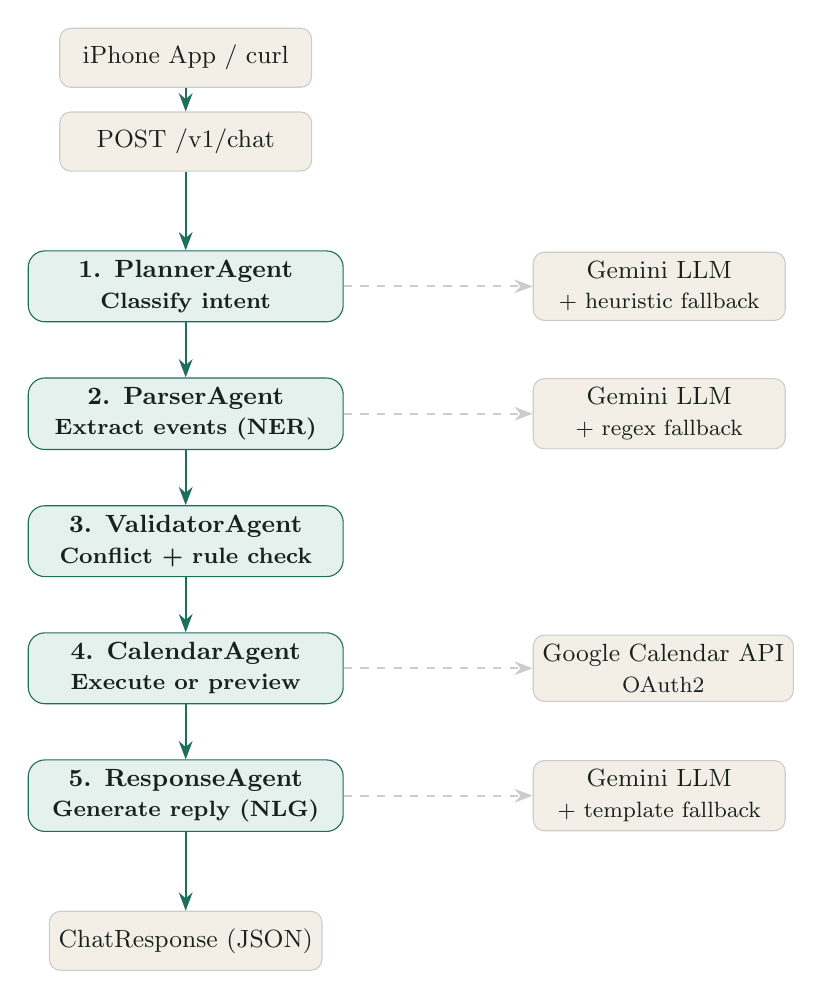
\begin{tikzpicture}[
  node distance=0.7cm and 1.0cm,
  box/.style={rectangle, rounded corners=6pt, draw=primary, fill=accent,
              minimum width=4.0cm, minimum height=0.9cm,
              font=\small\bfseries, text=secondary, align=center},
  extbox/.style={rectangle, rounded corners=4pt, draw=rulegray, fill=lightgray,
                 minimum width=3.2cm, minimum height=0.75cm,
                 font=\small, text=secondary, align=center},
  arr/.style={-Stealth, thick, color=primary},
  darr/.style={-Stealth, thick, color=rulegray, dashed},
]
\node[box] (planner)   {1. PlannerAgent\\{\footnotesize Classify intent}};
\node[box, below=of planner]  (parser)    {2. ParserAgent\\{\footnotesize Extract events (NER)}};
\node[box, below=of parser]   (validator) {3. ValidatorAgent\\{\footnotesize Conflict + rule check}};
\node[box, below=of validator](calendar)  {4. CalendarAgent\\{\footnotesize Execute or preview}};
\node[box, below=of calendar] (responder) {5. ResponseAgent\\{\footnotesize Generate reply (NLG)}};
\node[extbox, above=1.0cm of planner] (http) {POST /v1/chat};
\node[extbox, above=0.3cm of http]    (client) {iPhone App / curl};
\node[extbox, right=2.4cm of planner]  (llm1) {Gemini LLM\\{\footnotesize + heuristic fallback}};
\node[extbox, right=2.4cm of parser]   (llm2) {Gemini LLM\\{\footnotesize + regex fallback}};
\node[extbox, right=2.4cm of calendar] (gcal) {Google Calendar API\\{\footnotesize OAuth2}};
\node[extbox, right=2.4cm of responder](llm3) {Gemini LLM\\{\footnotesize + template fallback}};
\node[extbox, below=1.0cm of responder](resp) {ChatResponse (JSON)};
\draw[arr] (client)    -- (http);
\draw[arr] (http)      -- (planner);
\draw[arr] (planner)   -- (parser);
\draw[arr] (parser)    -- (validator);
\draw[arr] (validator) -- (calendar);
\draw[arr] (calendar)  -- (responder);
\draw[arr] (responder) -- (resp);
\draw[darr] (planner)   -- (llm1);
\draw[darr] (parser)    -- (llm2);
\draw[darr] (calendar)  -- (gcal);
\draw[darr] (responder) -- (llm3);
\end{tikzpicture}
\end{center}

\subsection{Latency Analysis}

\begin{warnbox}[Scalability concern: three serial LLM calls]
  Each request makes \textbf{three sequential LLM calls} (Planner $\to$ Parser $\to$ Responder). If each call takes 500ms, that is 1.5 seconds of pure LLM wait time per request, before any calendar I/O. This is acceptable for conversational UX but is a hard ceiling imposed by the sequential design. Stages 1 and 3 could potentially be parallelised (Planner and Responder do not depend on each other's output in the current design), but the current code runs them serially.
\end{warnbox}

\begin{table}[htbp]
\centering
\small
\renewcommand{\arraystretch}{1.4}
\begin{tabularx}{\textwidth}{L{3.5cm} L{2.5cm} X}
\toprule
\textbf{Stage} & \textbf{Typical latency} & \textbf{Bottleneck} \\
\midrule
PlannerAgent (LLM) & 300--600ms & Network RTT to Gemini API \\
ParserAgent (LLM)  & 400--800ms & Larger output schema \\
ValidatorAgent     & $<$1ms     & Pure Python logic, no I/O \\
CalendarAgent      & 200--400ms & OAuth token refresh + 1--N Google API calls \\
ResponseAgent (LLM)& 300--600ms & Network RTT to Gemini API \\
\midrule
\textbf{Total (LLM path)} & \textbf{1.2--2.4s} & LLM calls dominate \\
\textbf{Total (fallback)}  & \textbf{200--400ms} & Only Google Calendar I/O \\
\bottomrule
\end{tabularx}
\caption{Estimated latency per pipeline stage}
\end{table}

\subsection{Mental Model}

Think of Dayli as a \textbf{translation assembly line with a safety gate}. Raw English enters. Each station refines it: intent classification $\to$ entity extraction $\to$ rule validation $\to$ calendar write $\to$ natural language reply. The safety gate (\texttt{preview}/\texttt{apply}) lets you inspect the output before any external mutation occurs. If any station's AI component breaks, a simpler mechanical fallback takes over so the line never stops completely.


% ============================================================
\section{Core Design Principles \& Engineering Rigour}
% ============================================================

\subsection{The Five Key Design Decisions}

\subsubsection{1. Multi-Agent Sequential Pipeline (Separation of Concerns)}

Each of the five stages has exactly one job and a well-defined input/output contract. This is the \textbf{Single Responsibility Principle} applied at the service level.

\textbf{Why not one large prompt?} A single ``God prompt'' (``Given this message, return all events, validate them, and generate a reply'') has several failure modes: the output schema is complex and error-prone, a failure in one sub-task pollutes all sub-tasks, and the prompt is untestable. Separate agents allow each sub-task to be unit-tested, replaced, or swapped independently.

\textbf{The cost:} Three LLM calls instead of one. For latency-sensitive applications, this is a real trade-off. The current design accepts higher latency in exchange for modularity.

\subsubsection{2. LLM With Deterministic Fallback — Defence in Depth}

Every agent tries the LLM first and falls back to regex/heuristics on any exception. This is the \textbf{Circuit Breaker} pattern applied at the inference level.

\begin{lstlisting}[language=Python, caption={The fallback pattern -- repeated in all five agents}]
async def plan(self, message: str) -> PlanResult:
    try:
        response = await self._llm_client.chat.completions.create(...)
        return structured_result_from_llm(response)
    except Exception as exc:
        logger.warning("LLM failed (%s), using heuristic", exc)
        return self._heuristic(message)   # regex / rule-based backup
\end{lstlisting}

\textbf{The hidden cost:} \texttt{except Exception} is a blunt instrument. It catches everything: quota errors, network timeouts, model-not-found errors, \emph{and} programming bugs. In production, you need error classification:

\begin{itemize}
  \item \texttt{RateLimitError} $\to$ retry with exponential backoff
  \item \texttt{APIConnectionError} $\to$ fallback immediately
  \item \texttt{JSONDecodeError} $\to$ this is a prompt-engineering bug; alert, do not silently fall back
  \item \texttt{TypeError}/\texttt{KeyError} $\to$ programming bug; re-raise and surface it
\end{itemize}

\subsubsection{3. Preview Before Apply (Two-Phase Commit)}

Every request defaults to \texttt{mode="preview"}. The full pipeline runs, computing the complete change set, but nothing is written to Google Calendar until \texttt{mode="apply"} is explicitly sent.

\begin{lstlisting}[language=Python, caption={Calendar write gated on mode -- the safety valve}]
async def apply_changes(self, user_id: str, changes: ScheduleChangeSet) -> None:
    if changes.mode != "apply" or not changes.events:
        return    # <-- exits cleanly; no side effects
    access_token = await self._get_access_token()
    # ... POST to Google Calendar API
\end{lstlisting}

\textbf{Why this matters:} This pattern is essential for any system with irreversible external effects (calendar writes, email sends, database mutations). It makes the system safe to test in production with real credentials because the default behaviour causes no mutations. It also enables a UX where users review a ``plan'' before committing.

\subsubsection{4. Dependency Injection Over Global State}

Credentials and services are passed as constructor arguments. This follows the \textbf{Dependency Inversion Principle}: high-level modules (the pipeline) depend on abstractions, not concrete implementations.

The specific bug this prevents: \texttt{pydantic-settings} with \texttt{env\_file=".env"} loads values into the \texttt{Settings} object but does \emph{not} write them into \texttt{os.environ}. Code that calls \texttt{os.environ.get("KEY")} after \texttt{pydantic-settings} has loaded the \texttt{.env} file will get an empty string. Passing credentials explicitly through constructors makes this class of bug impossible.

\subsubsection{5. Abstract Provider Interface (Open/Closed Principle)}

\texttt{CalendarProvider} is an abstract base class. The pipeline is closed for modification (you never change \texttt{CalendarAgent}) but open for extension (you add \texttt{OutlookCalendarProvider} by writing one new file). This is the \textbf{Strategy} pattern applied to external service integration.

\subsection{Design Patterns Reference}

\begin{table}[htbp]
\centering
\small
\renewcommand{\arraystretch}{1.4}
\begin{tabularx}{\textwidth}{L{2.8cm} L{4.0cm} X}
\toprule
\textbf{Pattern} & \textbf{Where used} & \textbf{Why this choice} \\
\midrule
Pipeline
  & The 5-agent sequence
  & Single responsibility per stage; independently replaceable \\
Strategy
  & \texttt{CalendarProvider} ABC
  & Open/closed: new providers without changing existing code \\
Two-Phase Commit
  & \texttt{preview}/\texttt{apply} mode
  & Safe-by-default mutation of external systems \\
Circuit Breaker (partial)
  & \texttt{try/except} + fallback in agents
  & Prevents LLM failure from cascading to the user \\
Singleton
  & \texttt{@lru\_cache} on \texttt{get\_settings()}
  & Config loaded once; avoids repeated file I/O \\
Factory Method
  & \texttt{ConversationManager.\allowbreak bootstrap()}
  & Centralised wiring; single place to change dependencies \\
\bottomrule
\end{tabularx}
\caption{Design patterns and justification}
\end{table}

\subsection{Explicit Trade-Off Analysis}

\begin{table}[htbp]
\centering
\small
\renewcommand{\arraystretch}{1.4}
\begin{tabularx}{\textwidth}{L{3.5cm} L{4.0cm} X}
\toprule
\textbf{Decision} & \textbf{Benefit} & \textbf{Cost / Risk} \\
\midrule
3 LLM calls per request
  & Modular, testable, focused prompts
  & 3$\times$ latency vs.\ single call; 3$\times$ token cost \\
\texttt{except Exception} fallback
  & System never crashes on LLM failure
  & Programming bugs are silently swallowed \\
In-memory stubs for repositories
  & Zero setup for demo; clear interfaces defined
  & No persistence: session state lost on restart \\
OpenAI-compatible Gemini endpoint
  & Swap model with one config change
  & Locked to OpenAI chat-completion API shape; limits Gemini-native features \\
\texttt{Conversation\-Manager} per request
  & Simple, stateless handler code
  & Reconstructs all agents on every call; no connection pooling \\
Single-user Google OAuth token
  & Simple setup for prototype
  & Does not scale to multi-user; one token = one person's calendar \\
\bottomrule
\end{tabularx}
\caption{Explicit trade-offs in the current design}
\end{table}


% ============================================================
\section{ML/AI Principles}
% ============================================================

\subsection{Model Choice \& Why It Matters}

Dayli uses \textbf{Gemini 2.0 Flash} (or \texttt{gemini-2.0-flash-lite} depending on quota) via Google's OpenAI-compatible endpoint. The choice was driven by:

\begin{enumerate}
  \item \textbf{Cost:} Free tier available via Google AI Studio (vs. OpenAI GPT-4 at \$10+/M tokens).
  \item \textbf{Drop-in compatibility:} Gemini exposes an OpenAI-compatible REST API, meaning the \texttt{openai} Python SDK works unchanged. This reduces migration friction.
  \item \textbf{Structured output support:} \texttt{response\_format: \{type: json\_object\}} is supported, which is critical for the pipeline.
\end{enumerate}

\textbf{What was traded away:} Gemini's free tier has aggressive rate limits (requests-per-minute and daily quota). When quota is hit, all three agents fall back to heuristics. A GPT-4-turbo or Claude-3 deployment would have more headroom but at significantly higher cost.

\subsection{Prompt Engineering: Why Each Prompt Is Designed This Way}

\subsubsection{PlannerAgent: Zero-Shot Intent Classification}

The system prompt defines exactly four intent classes with descriptions and a rigid output schema. This is \textbf{zero-shot prompting}: no labelled examples are provided.

\begin{lstlisting}[language=Python, caption={PlannerAgent system prompt design}]
_SYSTEM = (
    "You are a scheduling intent classifier. "
    "Classify into exactly one of: create, edit, rebalance, clarify.\n"
    'Respond with valid JSON only: {"intent": "<type>", "summary": "<one sentence>"}'
)
\end{lstlisting}

\textbf{Why zero-shot works here:} Intent classification with 4 well-defined classes is a task that modern LLMs handle reliably without examples. The classes are semantically distinct enough that the model rarely confuses them. If accuracy were critical, you would move to \textbf{few-shot} (3--5 examples per class in the prompt) or \textbf{fine-tuning} on a labelled intent dataset.

\textbf{Why force JSON output:} The \texttt{response\_format: json\_object} parameter instructs the model to guarantee valid JSON output. Without it, the model might say ``Here is the JSON: \{...\}'' which breaks \texttt{json.loads()}. This is the primary source of LLM parse failures in production NLU pipelines.

\subsubsection{ParserAgent: Few-Shot NER via Schema Injection}

The parser injects today's date into the user content, giving the model temporal grounding:

\begin{lstlisting}[language=Python, caption={Date injection prevents temporal ambiguity}]
user_content = f"Today's date: {today}\n\nUser message: {message}"
\end{lstlisting}

\textbf{Why this is important:} Without grounding, ``tomorrow'' is unresolvable. LLMs have training data cutoffs and cannot know the current date at inference time. Injecting the date converts a temporally ambiguous problem into a concrete one.

\textbf{What is missing:} The prompt does not provide \textbf{examples} (few-shot). For edge cases like ``pencil me in for a chat with Sarah next Thursday at half three'', the model might fail or produce inconsistent datetime formats. Production systems would include 2--4 labelled examples in the prompt to constrain output format.

\subsubsection{Model Temperature \& Determinism}

The current code does not set a \texttt{temperature} parameter. The default for Gemini is typically 1.0 (high creativity). For a task like event extraction, lower temperature (0.1--0.3) would produce more consistent, deterministic outputs and reduce hallucinated event details. This is an untuned hyperparameter in the current codebase.

\begin{warnbox}[Untuned hyperparameter: temperature]
  At temperature 1.0, the parser might generate different event titles for the same input on repeated calls (``gym'' vs.\ ``Gym session'' vs.\ ``Morning workout''). For a calendar assistant, determinism is more desirable than creativity. Setting \texttt{temperature=0.1} in parser and planner agents would improve consistency at the cost of marginal creativity in the responder.
\end{warnbox}

\subsection{When the Heuristic Outperforms the LLM}

This is a counter-intuitive but important observation:

\begin{keybox}[The heuristic can be more reliable than the LLM for specific cases]
  For well-defined, narrow patterns (``Gym at 7am'', ``Move gym to tomorrow''), the regex heuristic in \texttt{\_extract\_events()} and \texttt{\_build\_edit\_events()} is \textbf{deterministic, zero-latency, and free}. The LLM adds value for complex, ambiguous, or multi-event inputs. A production system would route simple inputs through the heuristic and use the LLM only when complexity warrants it --- this is \textbf{learned routing} or \textbf{cascade classification}.
\end{keybox}

\subsection{Bias \& Reliability Considerations}

\begin{itemize}
  \item \textbf{Input bias:} The heuristic regex assumes English, 12-hour time format, and Western date conventions. ``Gym at 19:00'' (24-hour format) would be mishandled by \texttt{\_iso\_time()} which adds 12 hours to any hour $\leq 7$.
  \item \textbf{Output consistency:} Event titles from the LLM path are not normalised (``gym'' vs.\ ``Gym'' vs.\ ``Gym Session''). Without post-processing, identical events get different display names.
  \item \textbf{Hallucination risk:} The parser LLM might generate plausible-sounding but incorrect events. The current validator only checks for \emph{non-empty} event lists, not for \emph{plausible} event details. A parser that hallucinates ``Board Meeting 9am--5pm'' when the user said ``quick gym session'' would pass validation.
\end{itemize}

\subsection{Evaluation Strategy: What Is Missing}

The codebase has no automated evaluation loop for the ML components. A production deployment would need:

\begin{table}[htbp]
\centering
\renewcommand{\arraystretch}{1.4}
\begin{tabularx}{\textwidth}{L{3.5cm} X}
\toprule
\textbf{What to measure} & \textbf{How to measure it} \\
\midrule
Intent classification accuracy
  & Label 100 messages with ground-truth intents; compute precision/recall per class \\
Entity extraction F1
  & Label events in 50 messages; compute field-level F1 (title, start, end) \\
End-to-end calendar write correctness
  & For a fixed test set, compare written events to expected events \\
Fallback activation rate
  & Log every LLM failure; track \% of requests using heuristic path \\
Response latency P50/P95
  & Time each stage; alert if P95 $>$ 3 seconds \\
\bottomrule
\end{tabularx}
\caption{Evaluation metrics for a production ML pipeline}
\end{table}


% ============================================================
\section{Structural Breakdown}
% ============================================================

\subsection{Directory Map and Module Roles}

\begin{table}[htbp]
\centering
\small
\renewcommand{\arraystretch}{1.3}
\begin{tabularx}{\textwidth}{>{\ttfamily\raggedright\arraybackslash}p{5.8cm} X}
\toprule
\normalfont\textbf{Path} & \textbf{Role} \\
\midrule
apps/api/main.py
  & FastAPI entry point: CORS, lifespan, route registration \\
apps/api/routes/chat.py
  & \texttt{POST /v1/chat} handler; delegates to \texttt{ConversationManager} \\
apps/api/dependencies.py
  & DI factory: \texttt{get\_conversation\_}\allowbreak\texttt{manager()} wires dependencies \\
dayli/orchestration/\allowbreak conversation\_manager.py
  & Orchestrator: owns the pipeline; exposes \texttt{handle\_message()} and \texttt{bootstrap()} \\
dayli/agents/planner\_\allowbreak agent.py
  & Stage 1: Intent classification (LLM + keyword fallback) \\
dayli/agents/parser\_\allowbreak agent.py
  & Stage 2: Event NER (LLM + regex fallback) \\
dayli/agents/validator\_\allowbreak agent.py
  & Stage 3: Deterministic business rule validation \\
dayli/agents/calendar\_\allowbreak agent.py
  & Stage 4: \texttt{ParsedRequest} $\to$ \texttt{ScheduleChangeSet}; calls provider \\
dayli/agents/response\_\allowbreak agent.py
  & Stage 5: Natural language generation (LLM + template fallback) \\
dayli/tools/calendar/\allowbreak google.py
  & Infrastructure: OAuth2 token refresh + Google Calendar v3 REST \\
dayli/tools/calendar/base.py
  & Abstraction: \texttt{CalendarProvider} ABC --- the extension point \\
dayli/llm/client.py
  & Infrastructure: thin wrapper over \texttt{AsyncOpenAI} $\to$ Gemini \\
dayli/domain/models/
  & Domain models: pure data, no I/O \\
dayli/domain/services/
  & Domain logic: conflict checking, scheduling, soft edits \\
dayli/core/config.py
  & Config: \texttt{pydantic-settings} + \texttt{@lru\_cache} singleton \\
dayli/repositories/
  & Data layer: all stubs (\texttt{del} placeholders for real DB) \\
apps/mobile/App.tsx
  & React Native chat UI; sends \texttt{mode:"preview"} by default \\
\bottomrule
\end{tabularx}
\caption{Key files and their responsibilities}
\end{table}

\subsection{Data Models: The Pipeline's Type Contracts}

\begin{center}
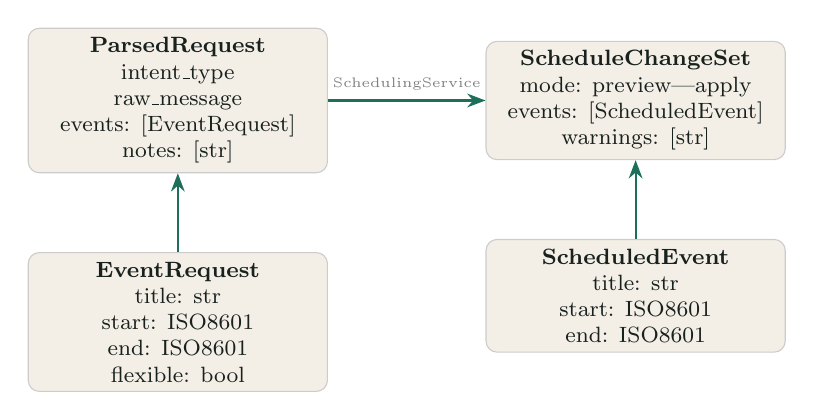
\begin{tikzpicture}[
  model/.style={rectangle, rounded corners=4pt, draw=rulegray, fill=lightgray,
                minimum width=3.8cm, minimum height=1.2cm,
                font=\footnotesize, text=secondary, align=center},
  arr/.style={-Stealth, thick, color=primary},
  lbl/.style={font=\tiny, color=gray, midway, above},
]
\node[model] (pr)  {\textbf{ParsedRequest}\\intent\_type\\raw\_message\\events: [EventRequest]\\notes: [str]};
\node[model, right=2.0cm of pr]  (sc) {\textbf{ScheduleChangeSet}\\mode: preview|apply\\events: [ScheduledEvent]\\warnings: [str]};
\node[model, below=1.0cm of pr]  (er) {\textbf{EventRequest}\\title: str\\start: ISO8601\\end: ISO8601\\flexible: bool};
\node[model, below=1.0cm of sc]  (se) {\textbf{ScheduledEvent}\\title: str\\start: ISO8601\\end: ISO8601};
\draw[arr] (pr) -- node[lbl]{SchedulingService} (sc);
\draw[arr] (er) -- (pr);
\draw[arr] (se) -- (sc);
\end{tikzpicture}
\end{center}

\textbf{Separation of concerns in the models:} \texttt{EventRequest} is mutable and carries the \texttt{flexible} flag for scheduling logic. \texttt{ScheduledEvent} is immutable and calendar-ready --- it has no \texttt{flexible} flag because by the time it reaches the calendar, that decision has been made. The transformation between them (\texttt{SchedulingService.to\_change\_set()}) is the point where scheduling decisions are locked in.


% ============================================================
\section{Conditional Knowledge --- When \& Why}
% ============================================================

\subsection{When Is Each Intent Used?}

\begin{table}[htbp]
\centering
\renewcommand{\arraystretch}{1.4}
\begin{tabularx}{\textwidth}{L{2.2cm} L{4.5cm} X}
\toprule
\textbf{Intent} & \textbf{Trigger signals} & \textbf{Pipeline action} \\
\midrule
\texttt{create}
  & ``schedule'', ``plan'', ``add'', \emph{or any default}
  & Parser extracts new events; all events are new \\
\texttt{edit}
  & ``move'', ``reschedule'', ``tomorrow'', ``shift''
  & Heuristic updates target event's time to +1 day, 18:00 \\
\texttt{rebalance}
  & ``less busy'', ``lighter'', ``free up''
  & Inserts a shifted ``Deep Work'' flexible block \\
\texttt{clarify}
  & Ambiguous request (LLM-detected)
  & \textbf{Bug:} currently falls through to \texttt{create}; should return a question \\
\bottomrule
\end{tabularx}
\caption{Intent types and their triggers}
\end{table}

\subsection{Failure Mode Taxonomy}

Understanding \emph{how} a system fails is as important as understanding how it works.

\begin{table}[htbp]
\centering
\small
\renewcommand{\arraystretch}{1.4}
\begin{tabularx}{\textwidth}{L{3.8cm} L{2.2cm} X}
\toprule
\textbf{Failure} & \textbf{Severity} & \textbf{Behaviour} \\
\midrule
Gemini quota exhausted
  & Degraded
  & All agents fall back to heuristics; system responds with lower quality \\
Google refresh token expired
  & Hard fail
  & \texttt{apply\_changes()} gets HTTP 401; no retry; user sees 500 \\
Malformed LLM JSON output
  & Degraded
  & Caught by \texttt{except Exception}; heuristic used silently \\
Empty event list from parser
  & Hard fail
  & \texttt{ConflictService} raises \texttt{ValidationError}; request fails \\
Manager rebuilt per request
  & Performance
  & Reconstructs 5 agents + HTTP client on every call; no pooling \\
No persistent memory
  & Feature gap
  & Context lost on restart; multi-turn references break \\
Single shared OAuth token
  & Scale limit
  & One token = one calendar; not multi-user \\
\bottomrule
\end{tabularx}
\caption{Failure modes, severity, and behaviour}
\end{table}

\subsection{When Would You Redesign Parts of This System?}

\begin{description}[leftmargin=1em, style=nextline]

  \item[If request volume exceeds 10 RPS]
    The synchronous sequential LLM pipeline becomes a bottleneck. You would redesign to: (a) parallelise Planner and an initial Responder skeleton; (b) cache frequent intent patterns; (c) use streaming responses to reduce perceived latency.

  \item[If multi-user support is needed]
    The single OAuth refresh token is replaced with a per-user token store. Each user goes through their own OAuth2 consent flow. Tokens are encrypted at rest in a database, not in a \texttt{.env} file.

  \item[If LLM accuracy is insufficient]
    You would add a labeled evaluation set, measure intent classification accuracy and entity F1, then decide: better prompts (few-shot), a smaller fine-tuned model (BERT-class for intent, T5 for NER), or a different base model (GPT-4-turbo, Claude 3 Opus).

  \item[If the heuristic fallback is producing wrong results]
    The regex in \texttt{\_extract\_events()} has a hard-coded date prefix (\texttt{2026-04-09}) and assumes 12-hour time. When the LLM is unavailable, all events get wrong dates. Fix: inject \texttt{date.today().isoformat()} into the heuristic, not just the LLM path.

  \item[If the \texttt{clarify} intent needs to work]
    The pipeline would need to break out of the single-request pattern: the responder would generate a clarifying question, the conversation manager would return without writing to the calendar, and the next user turn would be processed with the previous turn's context injected.

\end{description}

\subsection{The Limits of This Approach}

\begin{dangerbox}[Hard limits of zero-shot LLM prompting for scheduling]
  \begin{enumerate}
    \item \textbf{No user history:} The model cannot learn that ``this user always schedules gym at 6am'' because there is no persistent preference model. Each request starts cold.
    \item \textbf{No conflict awareness:} The validator does not fetch existing calendar events to check for conflicts --- it only validates the new events against each other.
    \item \textbf{No timezone intelligence:} All events are written in UTC. A user in Dubai scheduling ``gym at 7am'' gets an event at 07:00 UTC, which is 11am local time.
    \item \textbf{Hallucination at scale:} The LLM might fabricate event details with high confidence. There is no confidence score or calibration mechanism to detect uncertain outputs.
  \end{enumerate}
\end{dangerbox}


% ============================================================
\section{Procedural Knowledge --- How to Operate}
% ============================================================

\subsection{How to Run the Project}

\begin{lstlisting}[language=bash, caption={Full local setup from zero}]
# 1. Create and activate virtual environment
python -m venv .venv && source .venv/bin/activate

# 2. Install all dependencies (editable install)
pip install -e ".[dev]"

# 3. Copy config template and fill credentials
cp .env.example .env
# Edit .env: GEMINI_API_KEY, GOOGLE_CLIENT_ID, GOOGLE_CLIENT_SECRET

# 4. One-time: get Google OAuth2 refresh token
python scripts/google_auth.py
# Browser opens -> sign in -> paste GOOGLE_REFRESH_TOKEN into .env

# 5. Start the server
uvicorn apps.api.main:app --reload --port 8000

# 6. Preview (no calendar writes — safe to test)
curl -X POST http://localhost:8000/v1/chat \
  -H "Content-Type: application/json" \
  -d '{"user_id":"u1","session_id":"s1","message":"Gym at 7am","mode":"preview"}'

# 7. Apply to calendar (real write)
# Same command — change "mode":"preview" to "mode":"apply"
\end{lstlisting}

\subsection{How to Trace Execution Flow}

\begin{enumerate}
  \item \texttt{apps/api/routes/chat.py} $\to$ \texttt{chat()} receives the HTTP request
  \item \texttt{apps/api/dependencies.py} $\to$ \texttt{get\_conversation\_manager()} wires dependencies
  \item \texttt{dayli/orchestration/conversation\_manager.py} $\to$ \texttt{handle\_message()} runs the pipeline
  \item \texttt{dayli/agents/planner\_agent.py} $\to$ \texttt{plan()} classifies intent
  \item \texttt{dayli/agents/parser\_agent.py} $\to$ \texttt{parse()} extracts events
  \item \texttt{dayli/agents/validator\_agent.py} $\to$ \texttt{validate()} checks rules
  \item \texttt{dayli/agents/calendar\_agent.py} $\to$ \texttt{execute()} calls the provider
  \item \texttt{dayli/tools/calendar/google.py} $\to$ \texttt{apply\_changes()} writes to Google
  \item \texttt{dayli/agents/response\_agent.py} $\to$ \texttt{respond()} generates the reply
\end{enumerate}

\subsection{How to Debug Under Real-World Conditions}

\begin{table}[htbp]
\centering
\small
\renewcommand{\arraystretch}{1.45}
\begin{tabularx}{\textwidth}{L{3.8cm} L{3.8cm} X}
\toprule
\textbf{Symptom} & \textbf{Root cause} & \textbf{Fix} \\
\midrule
Generic event names (e.g.\ ``Updated event'')
  & Gemini quota exhausted; heuristic active
  & Check \texttt{GEMINI\_MODEL} in \texttt{.env}; verify quota in Google AI Studio \\
Calendar write silently skipped
  & \texttt{mode} is \texttt{"preview"} (default)
  & Send \texttt{"mode":"apply"} in the request body \\
Empty credentials at runtime
  & \texttt{os.environ.get()} bypasses pydantic-settings
  & Pass via constructor from \texttt{settings} object \\
\texttt{redirect\_uri\_}\newline\texttt{mismatch}
  & OAuth client is ``Web app'', not ``Desktop app''
  & Create a Desktop app OAuth 2.0 client in Google Cloud Console \\
\texttt{403 access\_denied}
  & App in Testing mode; user not in test users list
  & Add the user's Google account to the OAuth consent screen \\
Manager rebuilt on every request
  & \texttt{bootstrap()} called in DI factory, not at startup
  & Cache with \texttt{@lru\_cache} or move to app lifespan \\
Wrong dates (e.g.\ April 9 always)
  & Date hardcoded in heuristic \texttt{event.py}
  & Inject \texttt{date.today()} into heuristic path too \\
\bottomrule
\end{tabularx}
\caption{Production debugging guide}
\end{table}

\subsection{How to Scale This System Step-by-Step}

\begin{enumerate}
  \item \textbf{Fix the per-request object construction first.} Cache \texttt{ConversationManager} at app startup using FastAPI's lifespan context or \texttt{@lru\_cache}. This eliminates redundant object creation.

  \item \textbf{Add token caching for the Google OAuth access token.} Currently a fresh \texttt{POST} to \texttt{oauth2.googleapis.com/token} is made on every \texttt{apply} request. Access tokens are valid for one hour --- cache them with a TTL of 55 minutes.

  \item \textbf{Parallelise LLM calls where possible.} Planner and Responder do not depend on each other's output in the same request. They can be run concurrently with \texttt{asyncio.gather()}, cutting LLM latency by $\sim$30\%.

  \item \textbf{Add a real session store.} Replace \texttt{MemoryRepository} with Redis (for session state) and PostgreSQL (for audit logs). This enables multi-instance horizontal scaling.

  \item \textbf{Implement per-user OAuth.} Move from one shared token to a per-user token store. Encrypt tokens at rest. This is the gate to multi-tenant operation.

  \item \textbf{Add structured LLM output with retry.} Replace \texttt{response\_format: json\_object} with a \textbf{JSON schema-validated} approach (Instructor library or Pydantic AI). Add one retry with a corrective prompt on parse failure before falling back to heuristics.
\end{enumerate}

\subsection{How to Safely Extend the System}

\begin{description}[leftmargin=1em, style=nextline]
  \item[Add a new agent]
    Create \texttt{dayli/agents/my\_agent.py}. Register it in \texttt{ConversationManager.\_\_init\_\_}, \texttt{bootstrap()}, and \texttt{handle\_message()}.

  \item[Add a new calendar provider]
    Implement \texttt{CalendarProvider.apply\_changes()}. Change one line in the conversation manager:
    \begin{lstlisting}[language=Python]
provider: CalendarProvider = OutlookCalendarProvider(...)
    \end{lstlisting}

  \item[Add a new intent type]
    Add to \texttt{IntentType} in \texttt{dayli/core/types.py}. Handle it in the planner heuristic and in \texttt{ParsedRequest.from\_message()}.

  \item[Replace stubs with a real database]
    Implement \texttt{MemoryRepository} and \texttt{SessionRepository} using SQLAlchemy or Redis. The interface contracts are already defined.
\end{description}


% ============================================================
\section{Execution Flow --- End to End}
% ============================================================

The following traces a single request end-to-end, making every transition and decision point explicit.

\begin{center}
\texttt{\{"user\_id":"u1","session\_id":"s1","message":"Gym at 7am and work 9 to 5","mode":"apply"\}}
\end{center}

\begin{enumerate}[leftmargin=1.6cm, label=\textbf{Step \arabic*.}]

  \item \textbf{Load Context (ConversationMemory)}\\
    Returns \texttt{UserContext(user\_id="u1", timezone="UTC")}. Currently an in-memory stub --- returns a fresh context on every call. \textit{Cause $\to$ effect:} no persistent memory means multi-turn context (``move my earlier event'') cannot resolve ``earlier'' without prior conversation history.

  \item \textbf{Plan (PlannerAgent)}\\
    LLM receives: system prompt with 4 intent definitions + user message. Returns:
    \begin{lstlisting}[language={}]
{"intent": "create", "summary": "Schedule gym and work blocks"}
    \end{lstlisting}
    \textit{Fallback path:} \texttt{\_heuristic()} checks for ``move''/``reschedule'' keywords $\to$ \texttt{edit}; ``less busy'' $\to$ \texttt{rebalance}; default $\to$ \texttt{create}.

  \item \textbf{Parse (ParserAgent)}\\
    LLM receives: today's date injected + user message. Returns:
    \begin{lstlisting}[language={}]
{"events":[
  {"title":"Gym","start":"2026-04-16T07:00:00","end":"2026-04-16T08:00:00"},
  {"title":"Work","start":"2026-04-16T09:00:00","end":"2026-04-16T17:00:00"}
], "notes":[]}
    \end{lstlisting}
    Validated against \texttt{\_ParsedEvents} Pydantic model. \textit{Fallback:} regex scans for ``at HH'' and ``from HH to HH'' patterns.

  \item \textbf{Validate (ValidatorAgent)}\\
    \texttt{EditService.apply\_soft\_edits()} $\to$ no-op (stub).\\
    \texttt{ConflictService.ensure\_no\_conflicts()} $\to$ checks event list is non-empty.\\
    \textit{Gap:} does not check for time overlap with existing calendar events.

  \item \textbf{Execute (CalendarAgent)}\\
    \texttt{SchedulingService.to\_change\_set()} converts \texttt{ParsedRequest} into a \texttt{ScheduleChangeSet} with \texttt{mode="apply"}. Since mode is \texttt{"apply"}:
    \begin{enumerate}
      \item \textbf{Token refresh:} POST to Google's token endpoint with the stored refresh token; receives a fresh access token (1-hour TTL). No caching --- this call happens on \emph{every} apply request.
      \item \textbf{Event writes:} 2 sequential POST calls to the Google Calendar v3 events endpoint. Events appear in Google Calendar.
    \end{enumerate}

  \item \textbf{Respond (ResponseAgent)}\\
    LLM generates: \textit{``Your day is set! Gym at 7am and Work 9--5 are on your calendar.''}\\
    \textit{Fallback:} \textit{``Create schedule updates. I've added Gym, Work to your calendar.''}

  \item \textbf{Save \& Audit}\\
    Both \texttt{ConversationMemory.save()} and \texttt{AuditRepository.record()} are stubs (\texttt{del} the args). The hooks are structural placeholders for a real persistence layer.

  \item \textbf{Return}\\
    \begin{lstlisting}[language={}]
{
  "session_id": "s1",
  "reply": "Your day is set! ...",
  "changes": {
    "mode": "apply",
    "events": [{"title":"Gym",...}, {"title":"Work",...}],
    "warnings": []
  }
}
    \end{lstlisting}
\end{enumerate}


% ============================================================
\section{Critical Evaluation}
% ============================================================

\subsection{What Is Suboptimal or Fragile}

\begin{dangerbox}[The five most fragile points in the current design]
\begin{enumerate}
  \item \textbf{\texttt{except Exception} swallows programming bugs.} A \texttt{TypeError} inside an agent is treated the same as a Gemini rate limit. Both trigger the heuristic fallback silently. Production code should only catch expected external errors and let internal bugs propagate.

  \item \textbf{No OAuth token refresh for the calendar; no retry logic.} A single HTTP 401 from Google (expired access token) causes the entire request to fail with a 500. There is no retry-after-refresh logic.

  \item \textbf{Hardcoded dates in the heuristic fallback.} \texttt{date\_prefix = "2026-04-09"} in \texttt{\_extract\_events()} means that when the LLM is unavailable, all events land on April 9, 2026, regardless of when the request is made.

  \item \textbf{ConversationManager bootstrapped per request.} \texttt{dependencies.py} calls \texttt{ConversationManager.bootstrap(settings)} on every HTTP request. This constructs 5 agents, 2 services, 3 repositories, and 1 HTTP client per call. Under load, this is a significant memory and GC pressure issue.

  \item \textbf{Single-token architecture is not multi-user.} The system has one Google refresh token in \texttt{.env}. All calendar writes go to one person's calendar. This is a prototype constraint, not a bug, but it is the single most important limitation for any deployment beyond a personal demo.
\end{enumerate}
\end{dangerbox}

\subsection{What Would You Improve First and Why}

\begin{table}[htbp]
\centering
\small
\renewcommand{\arraystretch}{1.4}
\begin{tabularx}{\textwidth}{C{0.6cm} L{4.2cm} X L{1.8cm}}
\toprule
\textbf{\#} & \textbf{Improvement} & \textbf{Why first} & \textbf{Effort} \\
\midrule
1
  & Fix hardcoded date in heuristic (\texttt{date.today()})
  & Silent wrong-date bug; one-line fix; high user impact
  & 5 minutes \\
2
  & Cache \texttt{ConversationManager} at app startup
  & Performance; eliminates per-request object construction
  & 30 minutes \\
3
  & Cache Google access token with 55-minute TTL
  & Eliminates redundant OAuth call on every apply request
  & 1 hour \\
4
  & Classify exceptions in agents (not \texttt{except Exception})
  & Distinguishes bugs from external failures; critical for observability
  & 2 hours \\
5
  & Add retry-after-refresh for Google Calendar 401
  & Prevents hard failures on token expiry; standard OAuth pattern
  & 2 hours \\
6
  & Set \texttt{temperature=0.1} on Planner and Parser
  & More deterministic outputs; reduces LLM hallucination in NER
  & 10 minutes \\
7
  & Add real session storage (Redis)
  & Enables multi-turn context (``move my earlier event'')
  & 1 day \\
8
  & Implement per-user OAuth token store
  & Enables multi-user deployment
  & 3 days \\
\bottomrule
\end{tabularx}
\caption{Improvement roadmap ordered by impact/effort ratio}
\end{table}


% ============================================================
\section{Interview-Ready Framing}
% ============================================================

\subsection{``Explain Like I'm a Recruiter'' (60 seconds)}

\begin{interviewbox}[Recruiter narrative]
  Dayli is an AI-powered calendar assistant. Instead of tapping through menus to add events, you just describe your day in plain English: ``work from 9 to noon, gym at 6.'' The AI figures out what you mean, creates the calendar events, and asks for your confirmation before saving anything. It's built on top of Google's Gemini language model and connects directly to Google Calendar. I built the backend as a Python REST API and the frontend as an iPhone app. The interesting engineering challenge was making the system reliable even when the AI fails --- every component has a rule-based fallback so the app always responds, even if the AI is unavailable.
\end{interviewbox}

\subsection{``Explain Like I'm a Senior Engineer'' (2 minutes)}

\begin{interviewbox}[Senior engineer narrative]
  Dayli is a multi-agent NLU pipeline built on FastAPI with async Python. Each user message goes through five sequential stages: intent classification (create/edit/rebalance/clarify), named entity recognition for event extraction, deterministic rule validation, calendar provider execution, and natural language generation. Each stage calls Gemini via the OpenAI-compatible endpoint with structured output (\texttt{response\_format: json\_object}), and falls back to a regex/heuristic path on any exception. The calendar integration uses Google Calendar v3 via OAuth2 refresh token flow. The design follows a few explicit principles: single responsibility per agent, abstract provider interface for the calendar (Strategy pattern), and a preview/apply two-phase commit that makes the system safe-by-default. The current known weaknesses are: three serial LLM calls per request (1.5s+ latency), no persistent session memory (stubs only), per-request manager instantiation, and a single shared OAuth token that blocks multi-user deployment.
\end{interviewbox}

\subsection{``Explain Trade-offs in 60 Seconds'' (Technical Interview)}

\begin{interviewbox}[Trade-off narrative]
  The biggest design trade-off is three LLM calls per request instead of one. I chose separate agents for modularity and testability, but this triples latency and cost. Under load I'd parallelise the Planner and Responder stages with \texttt{asyncio.gather}. The second trade-off is \texttt{except Exception} everywhere for resilience --- the system never crashes, but it silently swallows programming bugs alongside external failures. I'd fix this by classifying exceptions: catch \texttt{RateLimitError} for backoff, catch \texttt{APIConnectionError} for fallback, and let everything else propagate. The third is using a single OAuth token in \texttt{.env} --- that's a prototype constraint that works for one user but requires a per-user encrypted token store to scale. Finally, the heuristic fallback has a hardcoded date, which is a silent correctness bug I'd fix before any production use.
\end{interviewbox}


% ============================================================
\section{Transferable Knowledge}
% ============================================================

\subsection{Reusable Principles}

\begin{keybox}[Principle 1 --- Pipeline over monolith for LLM workflows]
  When an LLM task decomposes into ordered discrete steps, a pipeline of focused agents is better than one mega-prompt. Each stage has a bounded context window, a testable contract, and can fail independently. The cost is latency and token count.
\end{keybox}

\begin{keybox}[Principle 2 --- Graceful degradation as a first-class concern]
  Every LLM call in a production system needs a deterministic fallback. The heuristic path is not a backup plan --- it is a peer path with guaranteed semantics. Design the fallback before the LLM path, not after.
\end{keybox}

\begin{keybox}[Principle 3 --- Two-phase commit for external mutations]
  Any system that writes to external systems (calendar, email, database) benefits from a preview/apply model. Default to preview. Require explicit confirmation. This makes the system safe to test with real credentials and builds user trust.
\end{keybox}

\begin{keybox}[Principle 4 --- Classify exceptions; never swallow bugs]
  \texttt{except Exception} is appropriate at the top level of a web handler. Inside a business logic component, it hides bugs. Know which exceptions represent external failures (retry/fallback) and which represent internal errors (propagate/alert).
\end{keybox}

\subsection{Reusable Patterns}

\begin{table}[htbp]
\centering
\small
\renewcommand{\arraystretch}{1.45}
\begin{tabularx}{\textwidth}{L{4.0cm} L{3.5cm} X}
\toprule
\textbf{Pattern} & \textbf{Where in Dayli} & \textbf{Reuse when} \\
\midrule
LLM + deterministic fallback
  & All 5 agents
  & Any LLM call in a production system \\
Abstract provider interface
  & \texttt{CalendarProvider} ABC
  & Supporting multiple implementations of one external service \\
\texttt{@lru\_cache} singleton config
  & \texttt{get\_settings()}
  & Config objects created exactly once per process \\
Pydantic for LLM output validation
  & \texttt{\_Classification}, \texttt{\_ParsedEvents}
  & Parsing structured JSON from any LLM \\
OAuth2 refresh-to-access flow
  & \texttt{Google\-Calendar\-Provider}
  & Any Google API requiring long-lived user credentials \\
Date injection in LLM prompt
  & ParserAgent
  & Any NLU task involving relative time expressions \\
\texttt{response\_format:}\newline\texttt{json\_object}
  & Planner, Parser
  & Getting reliable structured output from OpenAI-compatible models \\
\bottomrule
\end{tabularx}
\caption{Reusable patterns and when to apply them}
\end{table}

\subsection{Codebase Analysis Checklist}

Use this checklist to rapidly build understanding of any LLM-powered service:

\begin{itemize}[leftmargin=1.4cm, label=$\square$]
  \item What is the single job this system does? (What is its north-star metric?)
  \item How does a request enter and exit? (HTTP? Queue? File? What is the schema?)
  \item Is there a pipeline or a single handler? How many LLM calls per request?
  \item What is each prompt trying to achieve? What output schema is expected?
  \item What happens when the LLM fails? Is the fallback correct and tested?
  \item Where are external mutations? Is there a preview/dry-run mode?
  \item How are credentials loaded? Constructor injection or global state?
  \item Are LLM outputs validated? With Pydantic, JSON schema, or raw string parsing?
  \item What is stubbed vs.\ implemented? Where are the \texttt{del args} / TODO markers?
  \item What is the failure taxonomy? Which failures are degraded vs.\ hard?
  \item What would break first under 10$\times$ load? What is the scalability ceiling?
\end{itemize}

\subsection{Key Heuristics}

\begin{rulebox}
\begin{description}[leftmargin=1em, style=nextline, itemsep=6pt]
  \item[\faSearch\ Follow the request]
    Trace one HTTP request through the code. Every important file will appear.

  \item[\faExclamationTriangle\ Find the fallbacks]
    \texttt{except} blocks are your system's fragility map. What they catch tells you what the author feared.

  \item[\faTrash\ Find the \texttt{del}s]
    \texttt{del context} in stub methods = an explicit TODO. These are your integration debt map.

  \item[\faArrowRight\ Abstract class = extension point]
    Any ABC subclass (\texttt{CalendarProvider}) marks where the system is designed to grow.

  \item[\faCheckCircle\ Pydantic at the boundary]
    Every uncontrolled input (HTTP, LLM output) should hit a Pydantic model before entering business logic. Missing validation = reliability risk.

  \item[\faThermometerHalf\ No temperature = no control]
    If an LLM agent doesn't set temperature, its outputs are non-deterministic. For structured extraction tasks, always set a low temperature (0.1--0.3).
\end{description}
\end{rulebox}

\vspace{1.5cm}
\begin{center}
{\color{rulegray}\hrule height 0.4pt}\vspace{0.6cm}
{\small\color{gray} Dayli Senior Engineering \& ML/AI Report \textbullet\ Interview-ready edition \textbullet\ \today}
\end{center}

\end{document}
